\section{Log of \ref{sec:WBSTaskRepresentation} triple}

Task atomico, non suddiviso in sottotask.
\subsection{22/12/2009}
\paragraph{Esempio 1}
\paragraph{input}
\begin{figure}[h!]
\centering
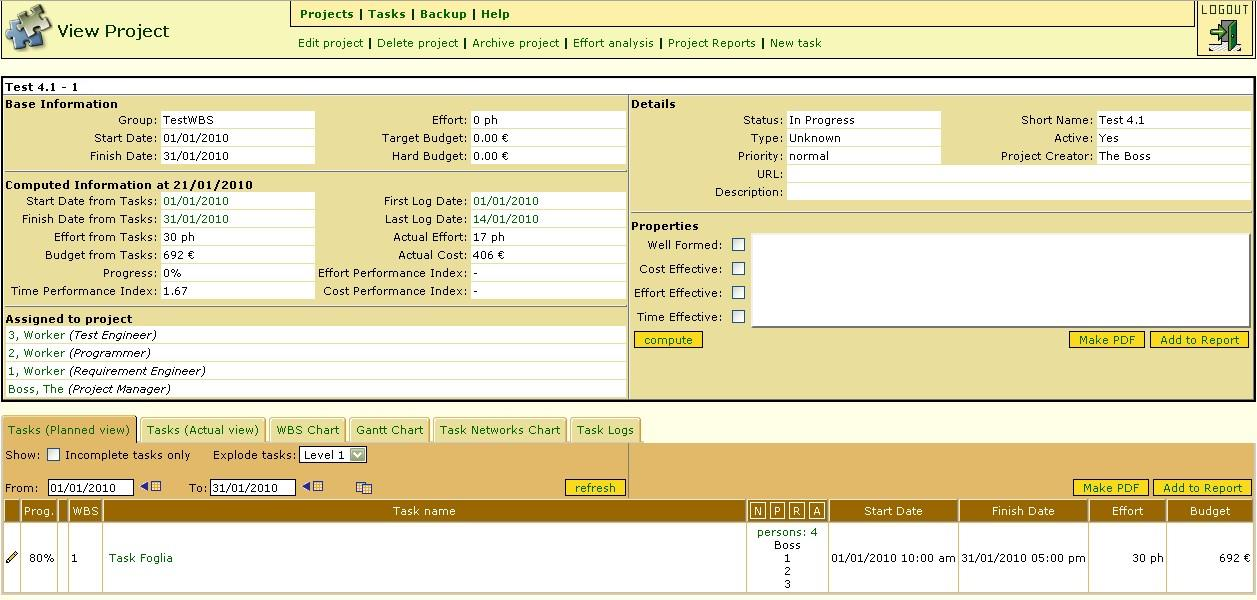
\includegraphics[width=\textwidth]{tests/TEST_WBS/4.1/4.1_1/Esempio_1/input.png}
\end{figure}
\begin{figure}[h!]
\centering
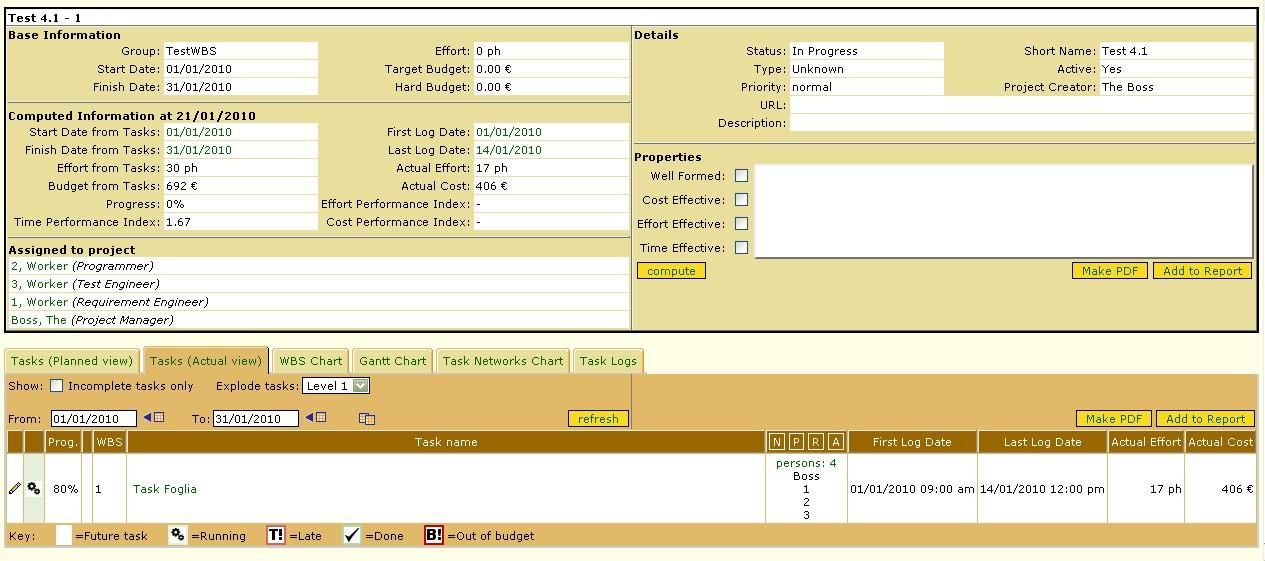
\includegraphics[width=\textwidth]{tests/TEST_WBS/4.1/4.1_1/Esempio_1/input_actual.png}
\end{figure}
\newpage
\paragraph{environment}
\begin{figure}
\centering
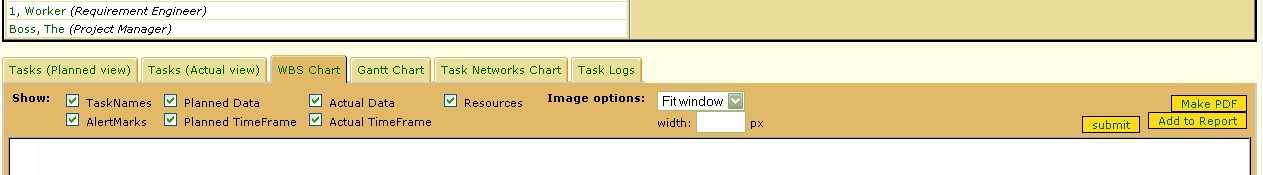
\includegraphics[width=\textwidth]{tests/TEST_WBS/4.1/4.1_1/Esempio_1/environment.png}
\end{figure}
\newpage
\paragraph{esito}
\begin{figure}
\centering

\includegraphics[width=\textwidth]{tests/TEST_WBS/4.1/4.1_1/Esempio_1/output.png}
\end{figure}
\newpage
\paragraph{Esempio 2}
\paragraph{input}
\begin{figure}
\centering
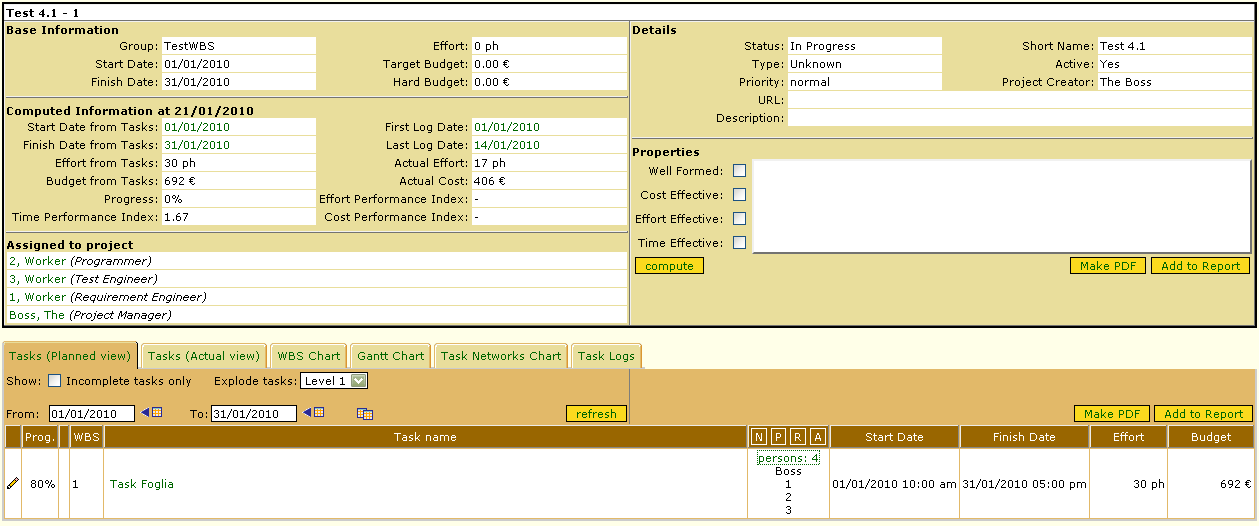
\includegraphics[width=\textwidth]{tests/TEST_WBS/4.1/4.1_1/Esempio_2/input.png}
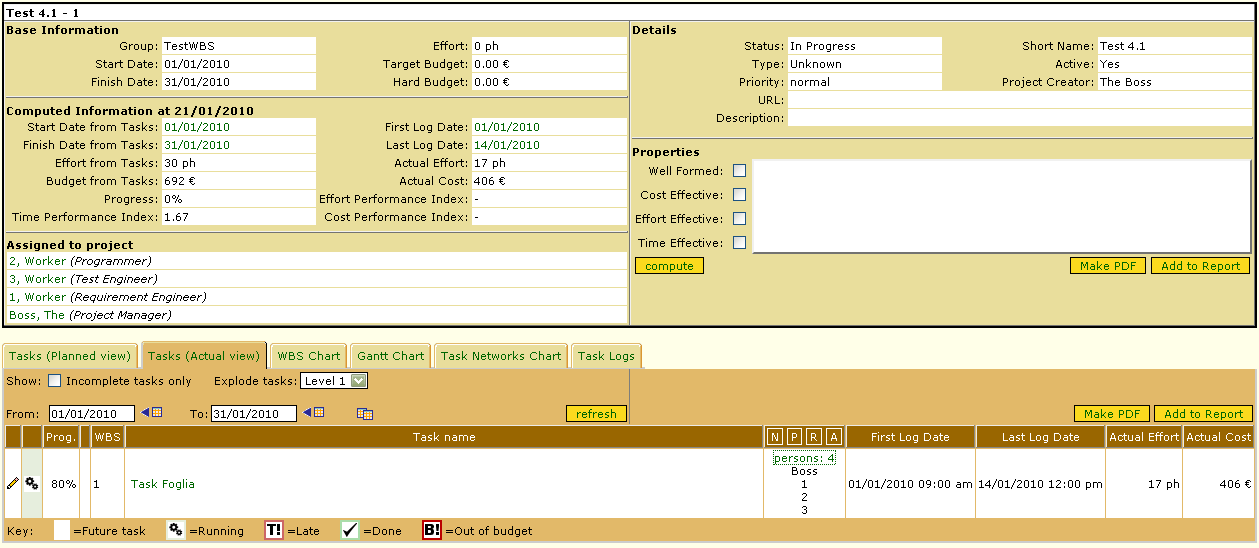
\includegraphics[width=\textwidth]{tests/TEST_WBS/4.1/4.1_1/Esempio_2/input_actual.png}
\end{figure}
\newpage
\paragraph{environment}
\begin{figure}
\centering
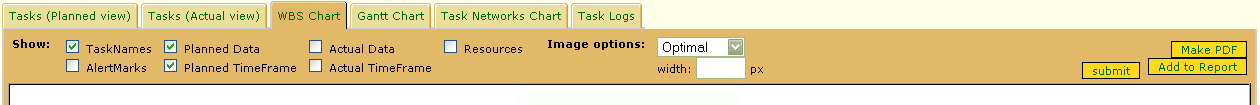
\includegraphics[width=\textwidth]{tests/TEST_WBS/4.1/4.1_1/Esempio_2/environment.png}
\end{figure}
\paragraph{esito}
\begin{figure}
\centering

\includegraphics[width=\textwidth]{tests/TEST_WBS/4.1/4.1_1/Esempio_2/output.png}
\end{figure}

\paragraph{Esempio 3}
\paragraph{input}
\begin{figure}
\centering
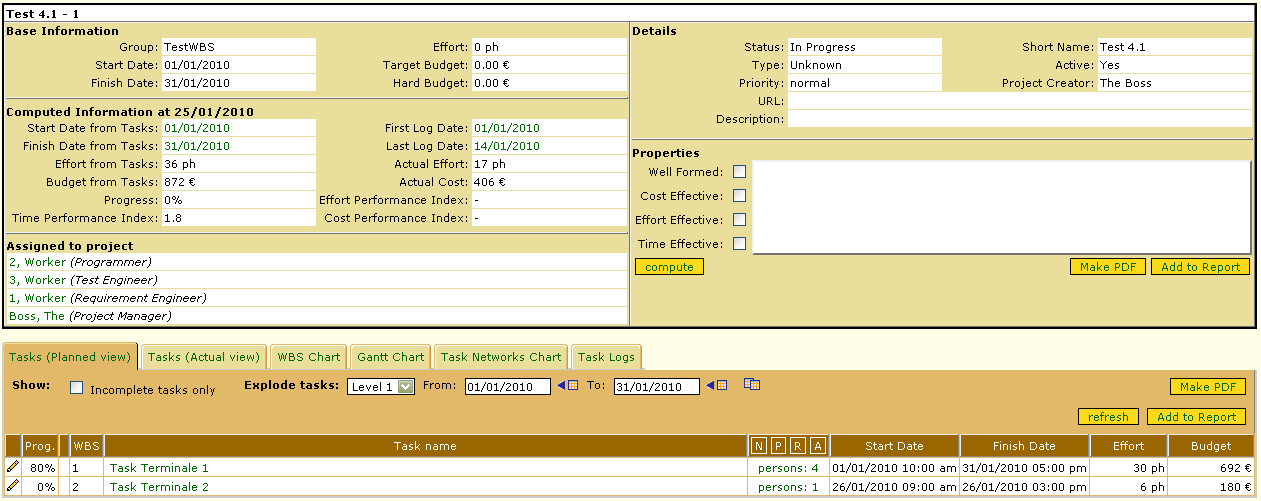
\includegraphics[width=\textwidth]{tests/TEST_WBS/4.1/4.1_1/Esempio_3/input.png}
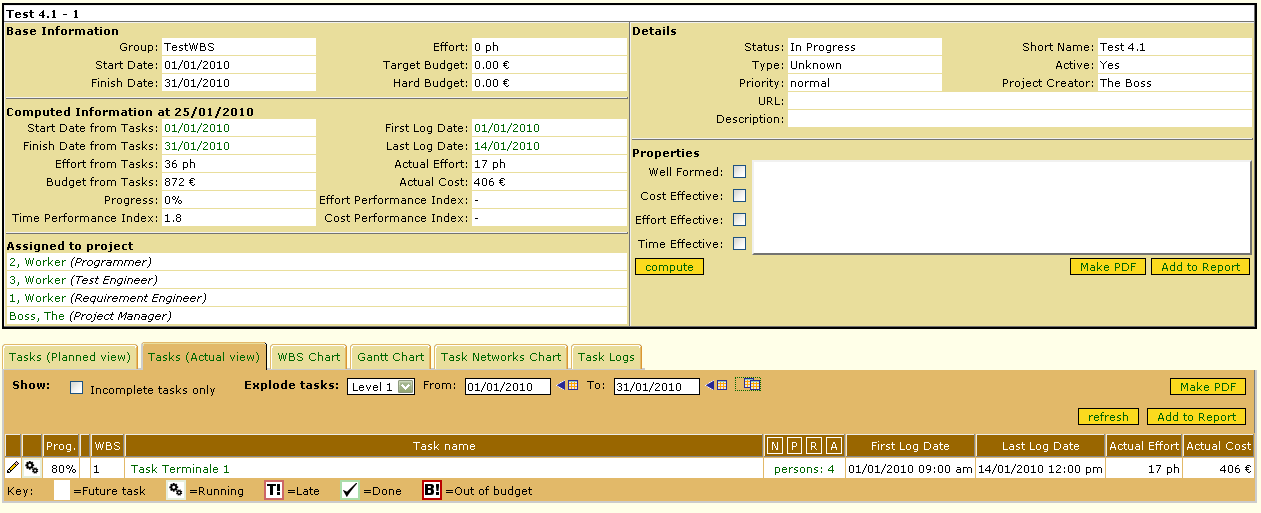
\includegraphics[width=\textwidth]{tests/TEST_WBS/4.1/4.1_1/Esempio_3/input_actual.png}
\end{figure}
\paragraph{environment}
\begin{figure}
\centering
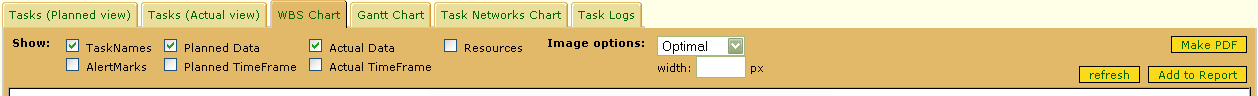
\includegraphics[width=\textwidth]{tests/TEST_WBS/4.1/4.1_1/Esempio_3/environment.png}
\end{figure}
\paragraph{esito}
\begin{figure}
\centering

\includegraphics[width=\textwidth]{tests/TEST_WBS/4.1/4.1_1/Esempio_3/output.png}
\end{figure}

Task composto, visualizzando i sotto task del livello successivo.

\subsection{22/12/2009}
\paragraph{Esempio 1}
\paragraph{input}
\begin{figure}
\centering
\includegraphics[width=\textwidth]{tests/TEST_WBS/4.1/4.1_2/Esempio_1/input.png}
\includegraphics[width=\textwidth]{tests/TEST_WBS/4.1/4.1_2/Esempio_1/input_actual.png}
\end{figure}
\paragraph{environment}
\begin{figure}
\centering
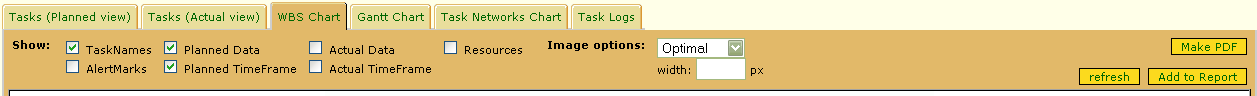
\includegraphics[width=\textwidth]{tests/TEST_WBS/4.1/4.1_2/Esempio_1/environment.png}
\end{figure}
\paragraph{esito}
\begin{figure}
\centering

\includegraphics[width=\textwidth]{tests/TEST_WBS/4.1/4.1_2/Esempio_1/output.png}
\end{figure}

\paragraph{Esempio 2}
\paragraph{input}
\begin{figure}
\centering
\includegraphics[width=\textwidth]{tests/TEST_WBS/4.1/4.1_2/Esempio_2/input.png}
\includegraphics[width=\textwidth]{tests/TEST_WBS/4.1/4.1_2/Esempio_2/input_actual.png}
\end{figure}
\paragraph{environment}
\begin{figure}
\centering
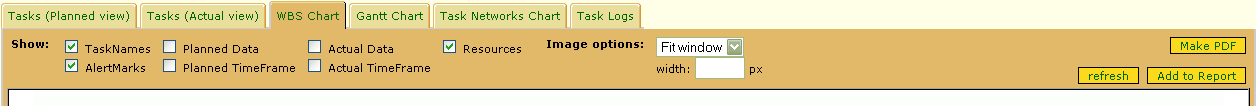
\includegraphics[width=\textwidth]{tests/TEST_WBS/4.1/4.1_2/Esempio_2/environment.png}
\end{figure}
\paragraph{esito}
\begin{figure}
\centering

\includegraphics[width=\textwidth]{tests/TEST_WBS/4.1/4.1_2/Esempio_2/output.png}
\end{figure}

Task composto, collassando i sotto task.

\subsection{22/12/2009}
\paragraph{Esempio 1}
\paragraph{input}
\begin{figure}
\centering
\includegraphics[width=\textwidth]{tests/TEST_WBS/4.1/4.1_3/Esempio_1/input.png}
\includegraphics[width=\textwidth]{tests/TEST_WBS/4.1/4.1_3/Esempio_1/input_actual.png}
\end{figure}
\paragraph{environment}
\begin{figure}
\centering
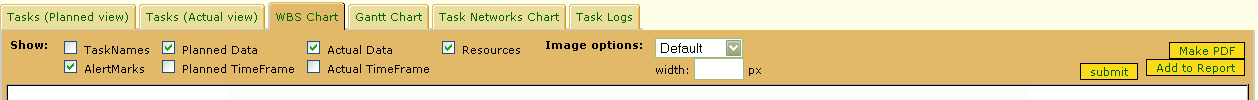
\includegraphics[width=\textwidth]{tests/TEST_WBS/4.1/4.1_3/Esempio_1/environment.png}
\end{figure}
\paragraph{esito}
\begin{figure}
\centering

\includegraphics[width=\textwidth]{tests/TEST_WBS/4.1/4.1_3/Esempio_1/output.png}
\end{figure}

\paragraph{Esempio 2}
\paragraph{input}
\begin{figure}
\centering
\includegraphics[width=\textwidth]{tests/TEST_WBS/4.1/4.1_3/Esempio_2/input.png}
\includegraphics[width=\textwidth]{tests/TEST_WBS/4.1/4.1_3/Esempio_2/input_actual.png}
\end{figure}
\paragraph{environment}
\begin{figure}
\centering
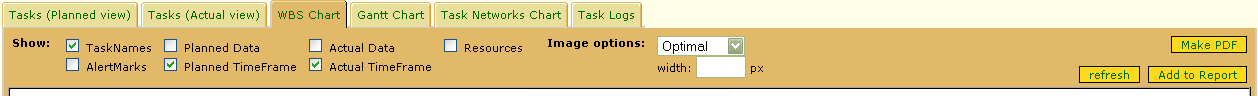
\includegraphics[width=\textwidth]{tests/TEST_WBS/4.1/4.1_3/Esempio_2/environment.png}
\end{figure}
\paragraph{esito}
\begin{figure}
\centering

\includegraphics[width=\textwidth]{tests/TEST_WBS/4.1/4.1_3/Esempio_2/output.png}
\end{figure}

Possibili varianti di task: coerenti, in anticipo, in ritardo, troppo costosi, non ancora loggati.

\subsection{22/12/2009}
\paragraph{Esempio 1}
\paragraph{input}
\begin{figure}
\centering
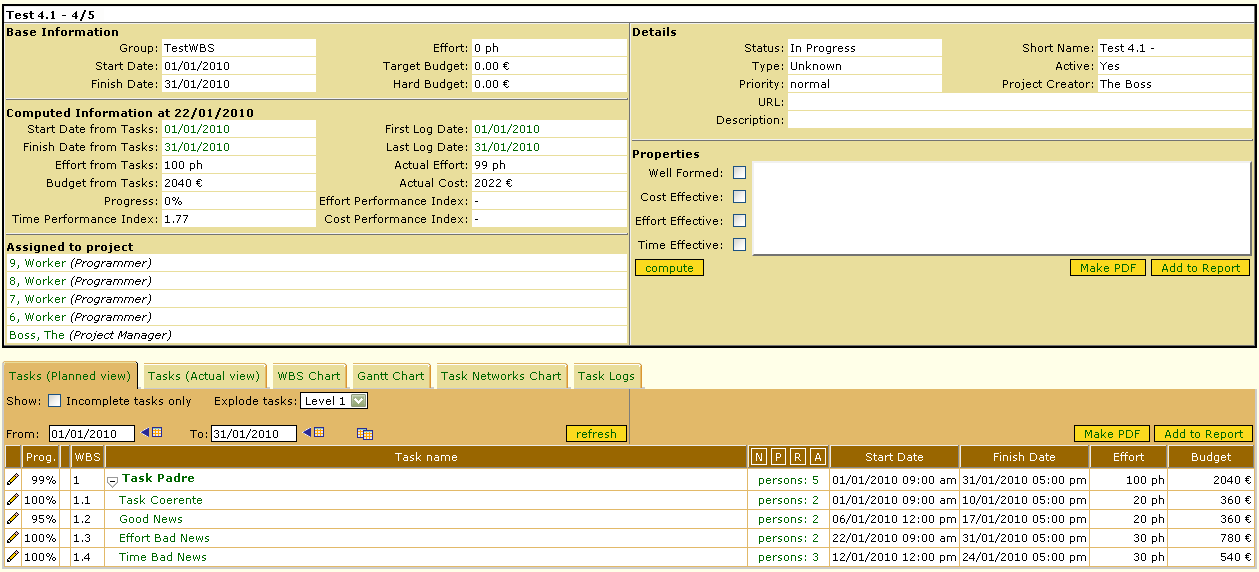
\includegraphics[width=\textwidth]{tests/TEST_WBS/4.1/4.1_4_5/Esempio_1/input.png}
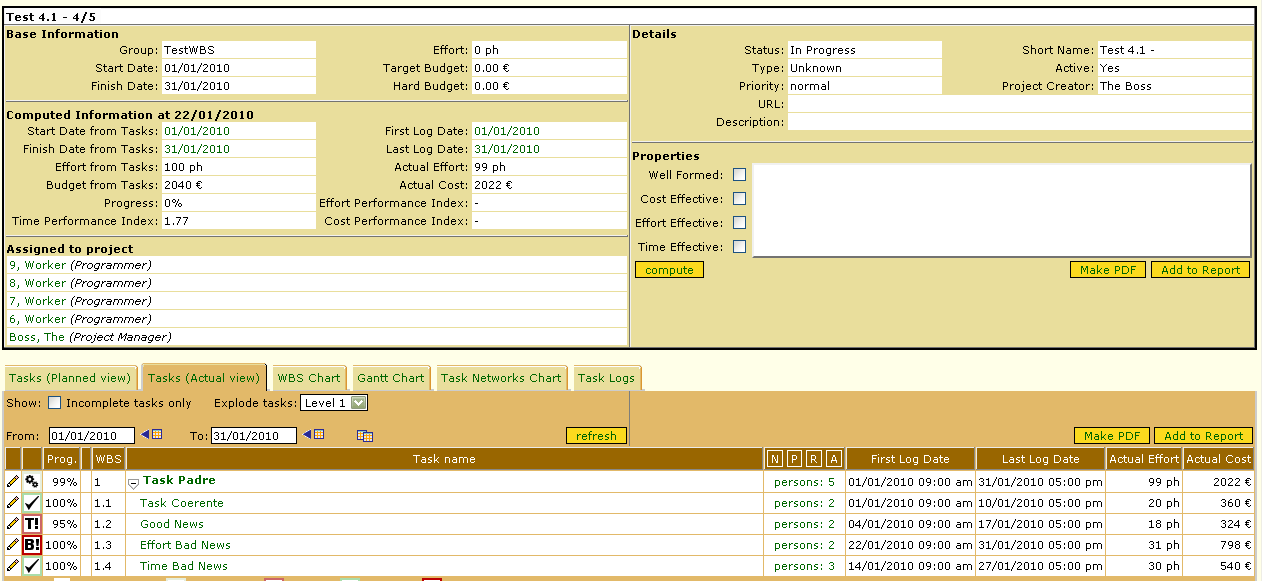
\includegraphics[width=\textwidth]{tests/TEST_WBS/4.1/4.1_4_5/Esempio_1/input_actual.png}
\end{figure}
\paragraph{environment}
\begin{figure}
\centering
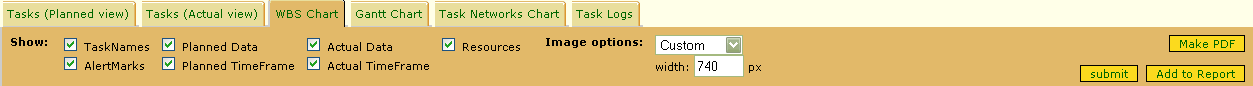
\includegraphics[width=\textwidth]{tests/TEST_WBS/4.1/4.1_4_5/Esempio_1/environment.png}
\end{figure}
\paragraph{esito}
\begin{figure}
\centering

\includegraphics[width=\textwidth]{tests/TEST_WBS/4.1/4.1_4_5/Esempio_1/output.png}
\end{figure}

\paragraph{Esempio 2}
\paragraph{input}
\begin{figure}
\centering
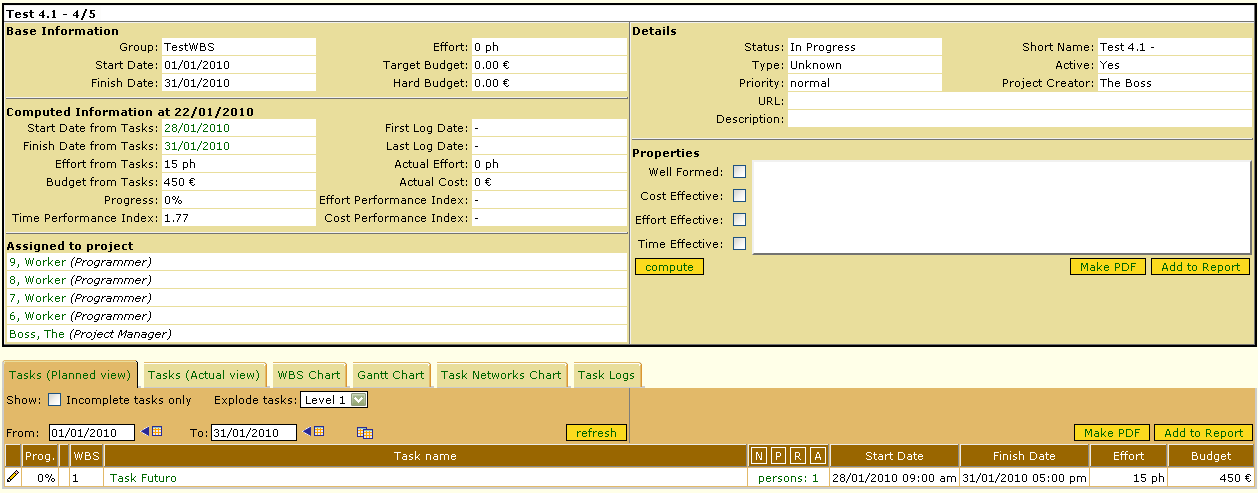
\includegraphics[width=\textwidth]{tests/TEST_WBS/4.1/4.1_4_5/Esempio_2/input.png}
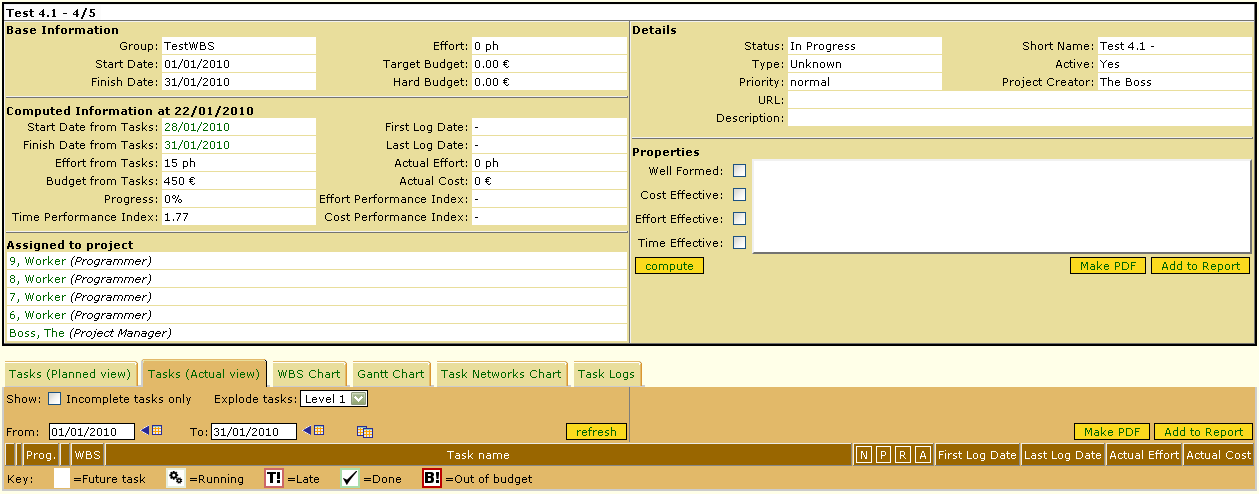
\includegraphics[width=\textwidth]{tests/TEST_WBS/4.1/4.1_4_5/Esempio_2/input_actual.png}
\end{figure}
\paragraph{environment}
\begin{figure}
\centering
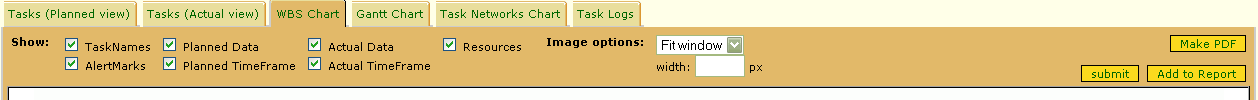
\includegraphics[width=\textwidth]{tests/TEST_WBS/4.1/4.1_4_5/Esempio_2/environment.png}
\end{figure}
\paragraph{esito}
\begin{figure}
\centering

\includegraphics[width=\textwidth]{tests/TEST_WBS/4.1/4.1_4_5/Esempio_2/output.png}
\end{figure}